
% Intended LaTeX compiler: pdflatex
\documentclass{article}

\usepackage{amsmath}
\usepackage{authblk}
\usepackage{graphicx}
\usepackage[hidelinks]{hyperref}
\usepackage{natbib}
\usepackage{tikz}
\usetikzlibrary{shapes}

\usepackage{todonotes}
\presetkeys{todonotes}{inline}{}

\date{}
% \title{Core Challenge 2022: Solver Tracks Documentation}
\title{(PARIS) Planning Algorithms for \\ Reconfiguring Independent Sets}
\pagenumbering{gobble}

\author[1]{Remo Christen}
\author[1]{Salomé Eriksson}
\author[2]{Michael Katz}
\author[3]{Emil Keyder}
\author[4]{Christian Muise}
\author[4]{Alice Petrov}
\author[1]{Florian Pommerening}
\author[5]{\\ Jendrik Seipp}
\author[1]{Silvan Sievers}
\author[6]{David Speck}

\affil[1]{University of Basel}
\affil[2]{IBM T.J. Watson Research Center}
\affil[3]{Invitae}
\affil[4]{Queen's University}
\affil[5]{Linköping University}
\affil[6]{University of Freiburg}

\newcommand{\astar}{\ensuremath{\text{A}^*}}
\renewcommand{\cite}[1]{\citep{#1}}

\begin{document}
\maketitle

\section{Introduction}
The general approach to all of the solver tracks was to model the ISR problem as one of automated planning, and use a selection of state-of-the-art solvers to solve these instances. Throughout this document, we describe the encoding, solvers, and overall search setup.

\section{Planning Encoding}

There are two main encodings we considered -- \textit{single} and \textit{split}. The former uses a single action to move a token from one location to another, while the latter uses two actions -- one to pick up a token and another to place it. While the full details on the Planning Domain Definition Language (PDDL) is out of scope for this document, the snippets presented here are fairly self-explanatory. More details on the PDDL standard can be found in \cite{pddlbook}.

\begin{figure}
    \centering
    \includegraphics[width=0.55\textwidth]{figures/move-single}
    \caption{PDDL example of a single action move.}
    \label{fig:move-single}
\end{figure}

Figure \ref{fig:move-single} shows the PDDL code for a single action move, with comments interleaved. Rather than define the actions in a lifted manner, we found that generating the ground actions (along with the conditions necessary to retain the independent set) was the most effective.

\begin{figure}[htbp]
  \centering
  \includegraphics[width=0.45\textwidth]{figures/move-split-pick}
  \hfill
  \includegraphics[width=0.45\textwidth]{figures/move-split-place}
  \caption{PDDL example of a pair of split actions for moving a token.}
  \label{fig:move-split}
\end{figure}

Figure \ref{fig:move-split} shows the pair of actions for the split encoding. Ultimately, we found this encoding to be the most effective, and so was used for all tracks and solvers.

Finally, the planning systems we used are all built on a common software framework which first parses and preprocesses the PDDL into an intermediate form known as SAS+ \cite{backstrom-nebel-compint1995}. To save on this computational effort, we instead directly encoded the input problem instances for the ISR contest into the SAS+ format. While in general this may lead to a degradation in performance (some planning problems benefit greatly from the preprocessing), in the ISR setting it was far more effective to skip this initial phase of planner technology.

\section{Engine: Core Solver or Algorithm}


We use sequential algorithm portfolios for each of the three solver tracks. That
is, we run a sequence of algorithms, each with an associated time limit. The
next section describes the algorithms that we use in our sequential portfolios.

\subsection{Our algorithms}

\paragraph{$\astar$+Landmarks} We run an $\astar$ search
\cite{hart-et-al-ieeessc1968} with a \emph{landmark count} heuristic
\cite{karpas-domshlak-ijcai2009} that uses two different kinds of landmarks:
$h^1$ landmarks \cite{keyder-et-al-ecai2010} and RHW landmarks
\cite{richter-et-al-aaai2008}. The landmark costs are combined with
\emph{uniform cost partitioning} \cite{katz-domshlak-icaps2008b}.

\paragraph{GBFS+Landmarks} We run a greedy best-first search (GBFS)
\cite{doran-michie-rsl1966} with a \emph{landmark count} heuristic
\cite{keyder-et-al-ecai2010} that computes all landmarks of the
\emph{delete-relaxed} task \cite{bonet-geffner-aij2001} ($h^1$ landmarks). The
landmark costs are combined with \emph{uniform cost partitioning}
\cite{katz-domshlak-icaps2008b}.

\paragraph{Symbolic search}
We run a forward symbolic blind search 
\cite{torralba-et-al-aij2017,speck-et-al-icaps2020} using Binary Decision 
Diagrams \cite{bryant-ieeecomp1986} as the underlying data structure. 
The symbolic planner we use is SymK \cite{speck-et-al-aaai2020}, which uses 
CUDD \cite{somenzi-cudd2015} as its decision diagram library. 
This algorithm is optimal, sound, and complete, i.e., if it reports a plan, 
this is a shortest plan, if it reports unsolvability, the task is indeed 
unsolvable, and given sufficient resources, it will eventually find a shortest 
plan.

\paragraph{Symbolic top-k search}
We run a modified forward symbolic blind search based on an algorithm 
called SymK-LL \cite{vontschammer-et-al-icaps2022}, implemented in the symbolic 
planner SymK \cite{speck-et-al-aaai2020}, which iteratively finds and generates 
all loopless plans of a given task.
However, we have made the following two major adjustments to solve the problem 
of finding the longest loopless plan feasible. 
First, once we find a goal state $s_{\star}$ reachable with a certain cost $c$, 
we reconstruct only one loopless plan with cost $c$ and ignore all other plans 
leading to $s_{\star}$ or any other goal state reachable with $c$. 
Second, since the split encoding introduced intermediate states in which a token 
is picked up, we ignore these artificial states when evaluating whether a plan 
is loopless during the plan reconstruction of SymK-LL.
This algorithm has the interesting property that it iteratively finds longer 
plans, starting with the shortest one, and eventually finds the longest loopless 
plan if enough resources are available.

\paragraph{Numeric abstraction} We abstract the problem to a numeric planning problem
and check for unsolvability in the abstraction. Since this algorithm is new, we describe
it in more detail in Section~\ref{sec:numeric-abstraction}.

We now describe our sequential algorithm portfolios. Our portfolio for the
\emph{existent} track is identical to the one for the \emph{shortest} track.

\subsection{Portfolio for \emph{shortest} and \emph{existent} tracks}

We list the algorithms and their time limits (the first to find a solution is saved and the rest of the steps ignored):

\begin{enumerate}
\item Numeric abstraction: 10sec
\item Symbolic search: 70min
\item $\astar$+Landmarks: 70min
\item GBFS+Landmarks: 70min
\item Numeric abstraction: 14hr
\end{enumerate}

\subsection{Single best solver for \emph{shortest} and \emph{existent} tracks}

The following single solver was used as a single-solver submission. It had the best coverage among all solvers in the portfolio.

\begin{itemize}
    \item GBFS+Landmarks: 70min
\end{itemize}

\subsection{Portfolio for \emph{longest} track}

We list the algorithms and their time limits:

\begin{enumerate}
\item GBFS+Landmarks: 330 seconds
\item Symbolic top-k search: 70min
\end{enumerate}

As a fall-back, if neither of the above approaches produced a solution longer than the shortest/existent track, we used the solution to the shortest/existent track as a default.

\subsection{Single best solver for \emph{longest} track}

The following single solver was used as a single-solver submission. It had the best coverage among all solvers in the portfolio. Note that we did not use the "fallback" option for this single track submission.

\begin{itemize}
    \item Symbolic top-k search: 70min
\end{itemize}

\section{Numeric Abstraction}
\label{sec:numeric-abstraction}

\begin{figure}[hb]
    \centering
    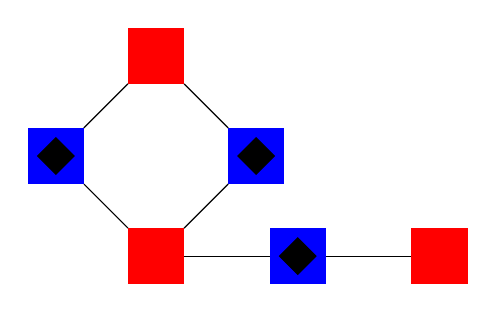
\begin{tikzpicture}[auto,node distance=18mm]
    \node[rectangle, minimum size=7mm, draw, fill, red]  (r1) {};
    \node[rectangle, minimum size=7mm, draw, fill, blue] (b1) [below left of=r1] {};
    \node[rectangle, minimum size=7mm, draw, fill, blue] (b2) [below right of=r1] {};
    \node[rectangle, minimum size=7mm, draw, fill, red]  (r2) [below left of=b2] {};
    \node[rectangle, minimum size=7mm, draw, fill, blue] (b3) [right of=r2] {};
    \node[rectangle, minimum size=7mm, draw, fill, red]  (r3) [right of=b3] {};

    \node[shape=diamond, draw, fill, black]  (t1) at (b1.center) {};
    \node[shape=diamond, draw, fill, black]  (t2) at (b2.center) {};
    \node[shape=diamond, draw, fill, black]  (t3) at (b3.center) {};

    \path (r1) edge (b1)
          (r1) edge (b2)
          (b1) edge (r2)
          (b2) edge (r2)
          (r2) edge (b3)
          (b3) edge (r3);
  \end{tikzpicture}
  \qquad
  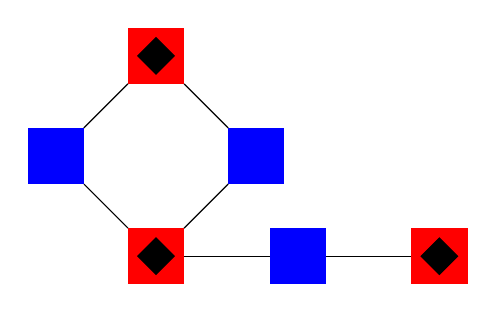
\begin{tikzpicture}[auto,node distance=18mm]
    \node[rectangle, minimum size=7mm, draw, fill, red]  (r1) {};
    \node[rectangle, minimum size=7mm, draw, fill, blue] (b1) [below left of=r1] {};
    \node[rectangle, minimum size=7mm, draw, fill, blue] (b2) [below right of=r1] {};
    \node[rectangle, minimum size=7mm, draw, fill, red]  (r2) [below left of=b2] {};
    \node[rectangle, minimum size=7mm, draw, fill, blue] (b3) [right of=r2] {};
    \node[rectangle, minimum size=7mm, draw, fill, red]  (r3) [right of=b3] {};

    \node[shape=diamond, draw, fill, black]  (t1) at (r1.center) {};
    \node[shape=diamond, draw, fill, black]  (t2) at (r2.center) {};
    \node[shape=diamond, draw, fill, black]  (t3) at (r3.center) {};

    \path (r1) edge (b1)
          (r1) edge (b2)
          (b1) edge (r2)
          (b2) edge (r2)
          (r2) edge (b3)
          (b3) edge (r3);
  \end{tikzpicture}

  \bigskip
  \bigskip
  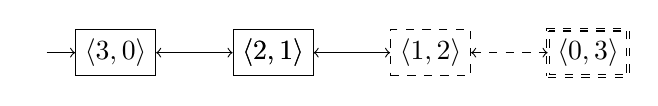
\begin{tikzpicture}[auto,node distance=2cm]
    \node (init) at (0, 0) {};
    \node[draw] (n30) at (1, 0) {$\langle 3,0 \rangle$};
    \node[draw] (n21) [right of=n30] {$\langle 2,1 \rangle$};
    \node[draw] (n21) [right of=n30] {$\langle 2,1 \rangle$};
    \node[draw,dashed] (n12) [right of=n21] {$\langle 1,2 \rangle$};
    \node[draw,dashed,double] (n03) [right of=n12] {$\langle 0,3 \rangle$};

    \path[draw,->] (init) edge (n30);
    \path[draw,<->] (n30) edge (n21);
    \path[draw,<->] (n21) edge (n12);
    \path[draw,<->,dashed] (n12) edge (n03);
  \end{tikzpicture}
  \caption{ Example coloring for numeric abstraction. The initial state is on
      the left and the goal state on the right. Nodes are colored blue if they have a
      token in the initial state but not the goal state and red if they have no token
      in the initial state but a token in the goal state. The abstract state space is
      shown below the instance. Dashed nodes are pruned.}
  \label{fig:numeric-abstractions-example}
\end{figure}

The \emph{numeric abstraction} component of our solver tries to detect if the
task is unsolvable by abstracting it to a numeric planning problem. Given an ISR
problem, we come up with a \emph{coloring} of the vertices in the graph, i.e., a
function that maps each vertex of the graph to one color. Many different ways of
coming up with a good coloring are conceivable but here we opted for a simple
strategy that uses up to four colors:
\begin{itemize}
    \item one for nodes that contain a token both in the initial state and in the goal state;
    \item one for nodes that contain a token only in the initial state but not in the goal state;
    \item one for nodes that contain a token only in the goal state but not in the initial state; and
    \item one for nodes that are empty in the initial state and goal state.
\end{itemize}

Colors for situations that do not occur are not used. For example, the task in
Figure~\ref{fig:numeric-abstractions-example} only requires two colors with the
method above.

Given a coloring, each configuration of tokens can be abstracted to a state with
one numeric variable per color that counts how many token currently are on
vertices with this color. For example, the initial state in
Figure~\ref{fig:numeric-abstractions-example} has 3 tokens on blue nodes and 0
on red nodes, so it can be represented as the numeric state $\langle 3,
0\rangle$. The goal state has all three tokens on red nodes and none on blue, so
it can represented by $\langle 0, 3 \rangle$.

Moving any token from a node colored $c_i$ to a node colored $c_j$ changes the
abstract state from $\langle c_1, \dots, c_i, \dots, c_j, \dots, c_n \rangle$ to
$\langle c_1, \dots, c_i-1, \dots, c_j+1, \dots, c_n \rangle$. The main
observation for this component is that if any solution to the full problem
exists, there has to be a solution in our abstraction as well. We thus construct
the state space of the abstraction in the following way.

For a state $s = \langle c_1, \dots, c_n \rangle$, we construct one successor
for each pair of different colors $c_i$ and $c_j$ that differs from $s$ by a
single token that moved from $c_i$ to $c_j$. In our running example, the initial
state $\langle 3, 0\rangle$ has a single successor $\langle 2, 1\rangle$, and
this state has two successors $\langle 3, 0\rangle$ (which we skip because we
have already seen this state) and $\langle 1, 2\rangle$. The latter state now
has the abstract goal state $\langle 0, 3\rangle$ as a successor (see
Figure~\ref{fig:numeric-abstractions-example}).

Whenever we generate a state, we check whether such a state is possible
(independent of whether we are actually able to reach such a state). If it is
not possible to place the token on the respective colors in the way suggest,
then we do not have to consider it or its successors. In our running example,
the state $\langle 1, 2 \rangle$ is not realizable: not matter where we place
the blue token, it blocks two of the three red nodes. We use a MIP solver to
check if a state $s$ is realizable by checking if the following system of
constraints have a solution:

\begin{align*}
    x_i + x_j &\le 1 \quad \text{for all edges $\langle i, j \rangle$ in the graph}\\
    \sum_{i \in N_c} x_i &\ge s[c] \quad \text{for all colors $c$} \\
    x_i \in \{0, 1\} & \qquad\text{for all nodes $i$}
\end{align*}
where $N_c$ is a set of all nodes with color $c$ and $s[c]$ is the amount of
tokens that should be on color $c$ in state $s$. The abstract state $s$ is realizable iff the
constraints have a solution.

If we generate a state that matches the goal state ($\langle 0, 3\rangle$ in our
example), we know that there is an abstract path to the goal state. In this case, we
still do not know if there is a real path to the goal state and return
\texttt{unknown} (this component of the solver is incomplete). However, if we
expand the full abstract state space without finding a path to an abstract goal
state, there is no solution to the abstract problem which also means there
cannot be a solution to the original problem. The abstract state space is
usually small. In our running example, it only has 4 states and we only have to
explore 3 of them, as we prune state $\langle 1, 2 \rangle$ before reaching a
goal state.

We use this component in two places: first with a small time limit at the start of
the solver to handle all cases where we can quickly prove unsolvability. Then
again with a large time limit after all other components to catch unsolvable
instances that are hard to prove unsolvable.


\section{Computation Environment}

All evaluations were conducted on a single machine running Ubuntu 20.04 (evaluations done through the Docker image for the submission), with the following specs:
\begin{itemize}
\item \textbf{CPU}: Intel(R) Xeon(R) Gold 5218 CPU @ 2.30GHz
\item \textbf{Cores}: 16
\item \textbf{MEM}: 128Gb
\end{itemize}



\bibliographystyle{abbrvnat}
\bibliography{abbrv-short,literatur,crossref-short,local}

\end{document}
